\documentclass[12pt]{article}
\usepackage{fullpage}
\usepackage{amsmath,amsthm,amssymb}
\usepackage{isotope}
% \usepackage[utf8]{inputenc}
% \usepackage[english]{babel}
\usepackage{graphicx,float}
\graphicspath{ {./img/} }

\theoremstyle{definition}
\newtheorem{prob}{Problem}[section]
\newtheorem{defn}{Definition}
\newtheorem*{ex}{Example}
\newtheorem*{soln}{Solution}

\newcommand{\K}{\frac{1}{4\pi\varepsilon_0}}
\newcommand{\abs}[1]{\left\vert#1\right\vert}
\newcommand{\e}[1]{\times10^{#1}}

\begin{document}
\title{Electromagnetism and Modern Physics}
\author{Mehedi Hasan}
\maketitle
\newpage
\section*{Preface}
This is not a holy text. So if there is a mistake, solve it by your own judgement.
\pagenumbering{roman}
\newpage
\tableofcontents
\newpage
\pagenumbering{arabic}
\section{Coulomb's Law}
\subsection{Coulomb's Torsion Balance Experiment}
\begin{figure}[h]
    \centering
    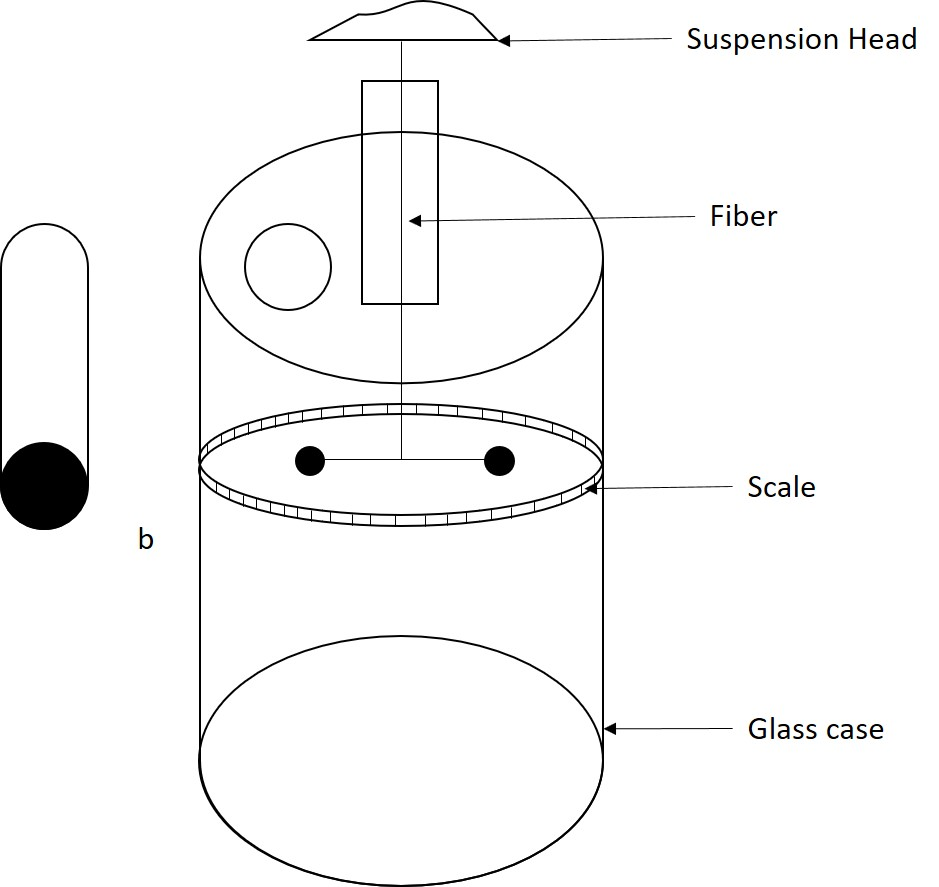
\includegraphics[scale=.5]{Picture1}
    \caption{Coulomb's torsion balance experiment}
    \label{fig:couTorsion}
\end{figure}
The force of attraction or repulsion between two point charges is directly proportional to the product of the charges and inversely proportional to the square of the distance between them. 

The direction of the force on each charged body is always along the line joining them,
\[F\propto \frac{q_1 q_2}{r^2}\Rightarrow\ F=\frac{K q_1 q_2}{r^2}\left| \begin{aligned}
    k &= \frac{1}{4\pi\varepsilon_0}\\
    &= 8.99\times10^9 Nm^2C^{-2}\\
    \varepsilon_0 &= 8.854\times10^{-12} C^{2}N^{-1}m^{-2}
\end{aligned}\right.\]
\newpage
\subsection{Vector form of Coulomb's Law}
\begin{figure}[h]
    \centering
    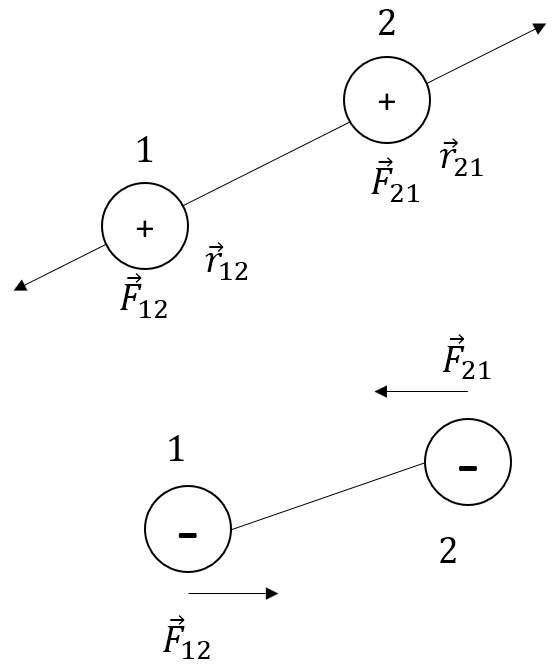
\includegraphics[scale=.5]{2.png}
    % \caption{}
    \label{fig:couVector}
\end{figure}
\begin{align*}
    \vec{F} &= \frac{kq_1q_2}{r^2}\hat{r}\\
    \vec{F} &= \frac{kq_1q_2}{r^3}\vec{r}\qquad \hat{r}=\frac{\vec{r}}{r}
\end{align*}
\begin{prob}
    Three charged particles held in places by forces (not shown in the figure). What electrostatic force owing to the other two charges acts on $ q_1 $? Where $ q_1 = -1.2\mu  $c, $ q_2=3.7\mu  $c, $ q_3=-2.3\mu  $c, $  r_{12}=15 $ cm, $  r_{13}=10 $ cm and $ \theta = 32^\circ $ 
    \begin{figure}[h]
        \centering
        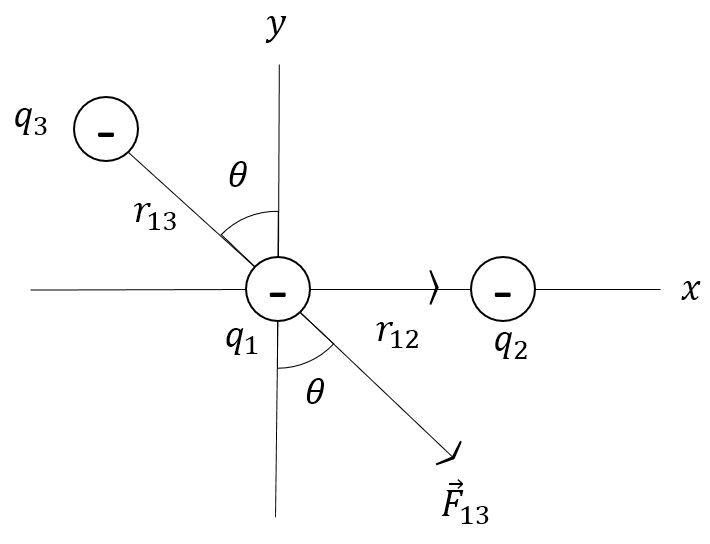
\includegraphics[scale=.5]{3.png}
        % \caption{}
        \label{fig:prob1}
    \end{figure}
\end{prob}
\begin{soln}
    Let us compute the magnitudes of the forces that $ q_2 $ and $ q_3 $ exert on $ q_1 $.
    \begin{align*}
        F_{12} &=\ \K \frac{\abs{q_1q_2}}{r_{12}^2}\\
         &=\ 8.99\times10^9 Nm^2C^{-2} \frac{\abs{-1.2\e{-6}c\cdot 3.7\e{-6}c}}{15\e{-2}}\\
         &=\ 1.77 \text{ N}
    \end{align*}
    Again, 
    \begin{align*}
        F_{13} &=\ \K \frac{\abs{q_1q_3}}{r_{13}^2}\\
         &=\ 8.99\e{9} Nm^2C^{-2} \frac{\abs{-1.2\e{-6}c\cdot -2.3\e{-6}c}}{10\e{-2}}\\
         &=\ 2.48 \text{ N}
    \end{align*}
    The component of resultant forces $ F_1 $ acting on $ q_1 $ are determined by the corresponding components.\\
    $ F_{1x}=\ F_{12x}+F_{13x}=\ 1.77+ (2.48\  \sin 32^\circ)=\ 3.08 $N\\
    $ F_{1y}=\ F_{12y}+F_{13y}=\ 0- (2.48\  \cos 32^\circ)=\ -2.10 $N\\
    From the components we can find the magnitude amd direction of $ \vec{F}_1 $.
    \begin{align*}
        F_1 &=\ \sqrt{{F_{1x}}^2+{F_{1y}}^2}\\
        &=\ \sqrt{3.08^2 N+(-2.10)^2 N}\\
        &=\ 3.73 N\\
        \intertext{and,}
        \theta &=\ \tan^{-1} \frac{F_{1y}}{F_{1x}}\\
        &=\ \tan^{-1} \frac{-2.10 N}{3.08 N}\\
        &=\ -34^\circ
    \end{align*}
    $ \vec{F}_1 $ vector makes an angle of $ -34^\circ $ with x-axis
\end{soln}
\begin{prob}
    What is the total force expected by the two charges on the charge $ q_3 $ located at origin? Where, $ q_1=2\e{-9} $c, $ q_2=-3\e{-9} $c and $ q_3=5\e{-9} $c.
    \begin{figure}[h]
        \centering
        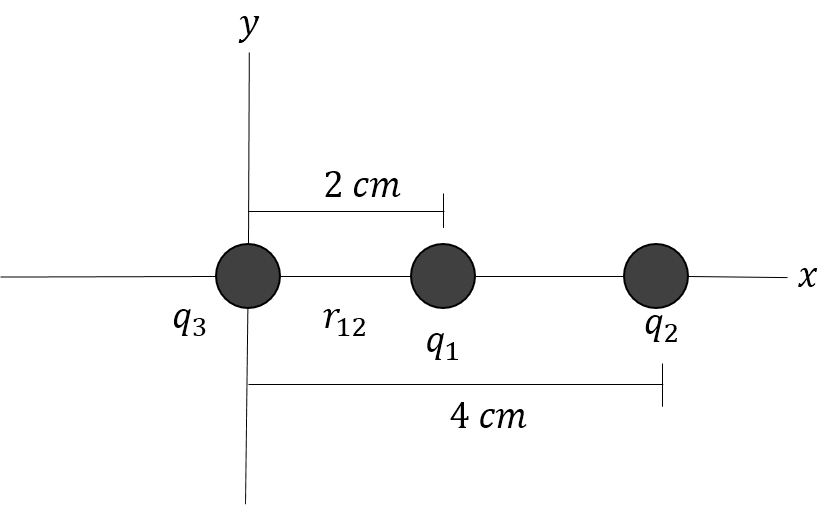
\includegraphics[scale=.5]{4.png}
        % \caption{}
        \label{fig:prob2}
    \end{figure}
\end{prob}
\begin{soln}
    TODO::Solve this 
\end{soln}
\begin{prob}
    Find the magnitude and direction of the total force on Q. Where, $ q=20\e{-6} $c and $ Q=4.0\e{6} $c.
    \begin{figure}[H]
        \centering
        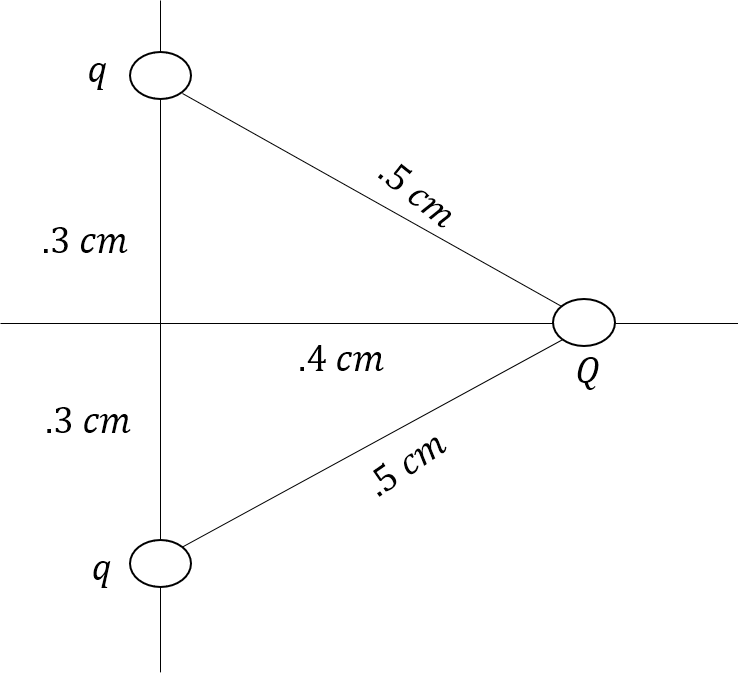
\includegraphics[scale=.5]{5.png}
        % \caption{}
        \label{fig:prob3}
    \end{figure}
\end{prob}
\begin{soln}
    TODO::Solve this 
\end{soln}
\subsection{Charge is Quantized}
When a physical quantity such as charge exists only in discrete 'packets' rather than incontinously variable amounts we that quantity is quantized.

Any charge $ q $ can be measured from $ q=ne;\ n=0,\pm1,\pm2,\dots $ Where $ e $ is the unit of elementary charge $ e=1.6\e{-19} $c. $ q=1.2e $ is not correct but $ q=1.2\mu c $ is correct.

up quark has $ +2/3 $e and down quark has $ -1/3 $e charge.\\
Proton $\displaystyle \to +\frac{2}{3}e\times2+ -\frac{1}{3}e=\ \frac{4}{3}-\frac{1}{3}=\frac{3}{3}=1 $\\
Neutron $\displaystyle \to +\frac{2}{3}e\times2+ -\frac{1}{3}\times2e=\ \frac{2}{3}-\frac{2}{3}=0 $\\

There is no evidence for the release of a free quark. A group of quarks are bounds so strongly in protons and neutrons and give the electrical charge in units of "$ e $".
\subsection{Charge is Conserved}
\begin{align*}
    \isotope[2]{H}+\isotope[2]{H} &\to\ \isotope[3]{H}+ P\\
    \isotope[2]{H}+\isotope[2]{H} &\to\ \isotope[4]{He}+ n\\
    e^+ +e^- &\to\ \gamma
\end{align*}
\section{Electric Field or Electric Field Intensity}
Coulomb's law $ \to $ charge $ \rightleftharpoons $ charge.\\
Introducing the field as an intermediary between charges. charge $ \rightleftharpoons $ field $ \rightleftharpoons $ charge.\\
The first charge sets up an electric field and the second charge interacts with the electric field on the first charge.
\begin{figure}[h]
    \centering
    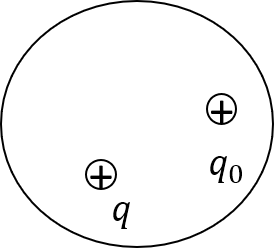
\includegraphics{6.png}
    % \caption{}
    % \label{}
\end{figure}
\begin{align*}
    q_0 \text{\----}\text{\----} &\ F\\
    1 \text{\----}\text{\----} &\ \frac{F}{q_0}
\end{align*}
\[E=\frac{F}{q_0}=\K \frac{q}{r^2}\]
\begin{figure}[h]
    \centering
    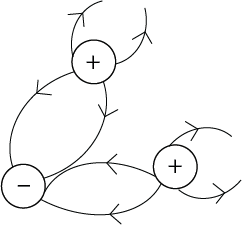
\includegraphics[scale=.5]{7.png}
    % \caption{}
    % \label{}
\end{figure}
\section{Electric Dipole}
\begin{figure}[h]
    \centering
    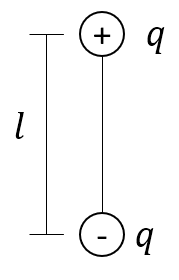
\includegraphics[scale=.75]{8.png}
    % \caption{}
    % \label{}
\end{figure}
A positive and negative charge of equal magnitude $ q $ placed a distance $ l $ apart, this configuration is called electric dipole.
\section{Electric Dipole in a Electric Field}
\begin{figure}[H]
    \centering
    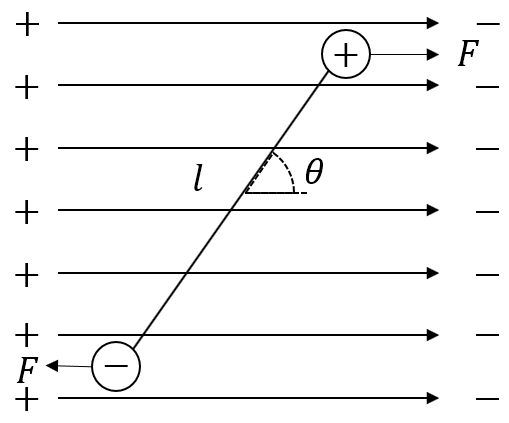
\includegraphics[scale=.75]{9.png}
    % \caption{}
    % \label{}
\end{figure}
Net force zero.\\ There is net torque about its center of mass that tends to rotate the dipole to bring alignment with $ \vec{E} $.\\
The magnitude of net torque,
\begin{align*}
    \tau &=\ F\frac{l}{2}\sin \theta +F\frac{l}{2}\sin \theta \\
    &=\ F \ l\ \sin \theta \\
    &=\ q\ E\ l\sin \theta\\
    &=\ q\ l\ E\sin\theta\\
    &=\ p\ E\sin\theta\\
    \vec{\tau}&=\ \vec{p}\times\vec{E}  \qquad [\because  \vec{\tau}=\vec{r}\times\vec{F}]
\end{align*}
\end{document}